%% BOUNDS
%%

In the cases of criteria C, E and F, we have derived a hard boundary on the 
isolated LDCs; for example, $c_2>0$ from criterion C. However, it is also useful 
to know about the other extrema; for example, what is the maximum bound on 
$c_2$? Working in the $\{c_2,c_3,c_4\}$ parameter space, which we refer 
to as the ``original'' reference frame, these bounds define the smallest cuboid 
within which the allowed loci reside.

\subsection{$c_3$-$c_2$ plane}
\label{sub:c3c2plane}

Starting from the seven criteria, how can we calculate the limits on each LDC?
We choose to proceed by means of numerically-guided analytic reasoning via
inspection of the projected 2D planes. 

We begin by generating a large number of random points drawn uniformly in 
$\{c_2,c_3,c_4\}$ and then reject any point which does not satisfy criteria A-G. 
The surviving points are then saved. We plot the loci of these points on the 
$c_3$-$c_2$ plane in Fig.~\ref{fig:c3c2surface}.

%%% c3-c2 surface
\begin{figure}
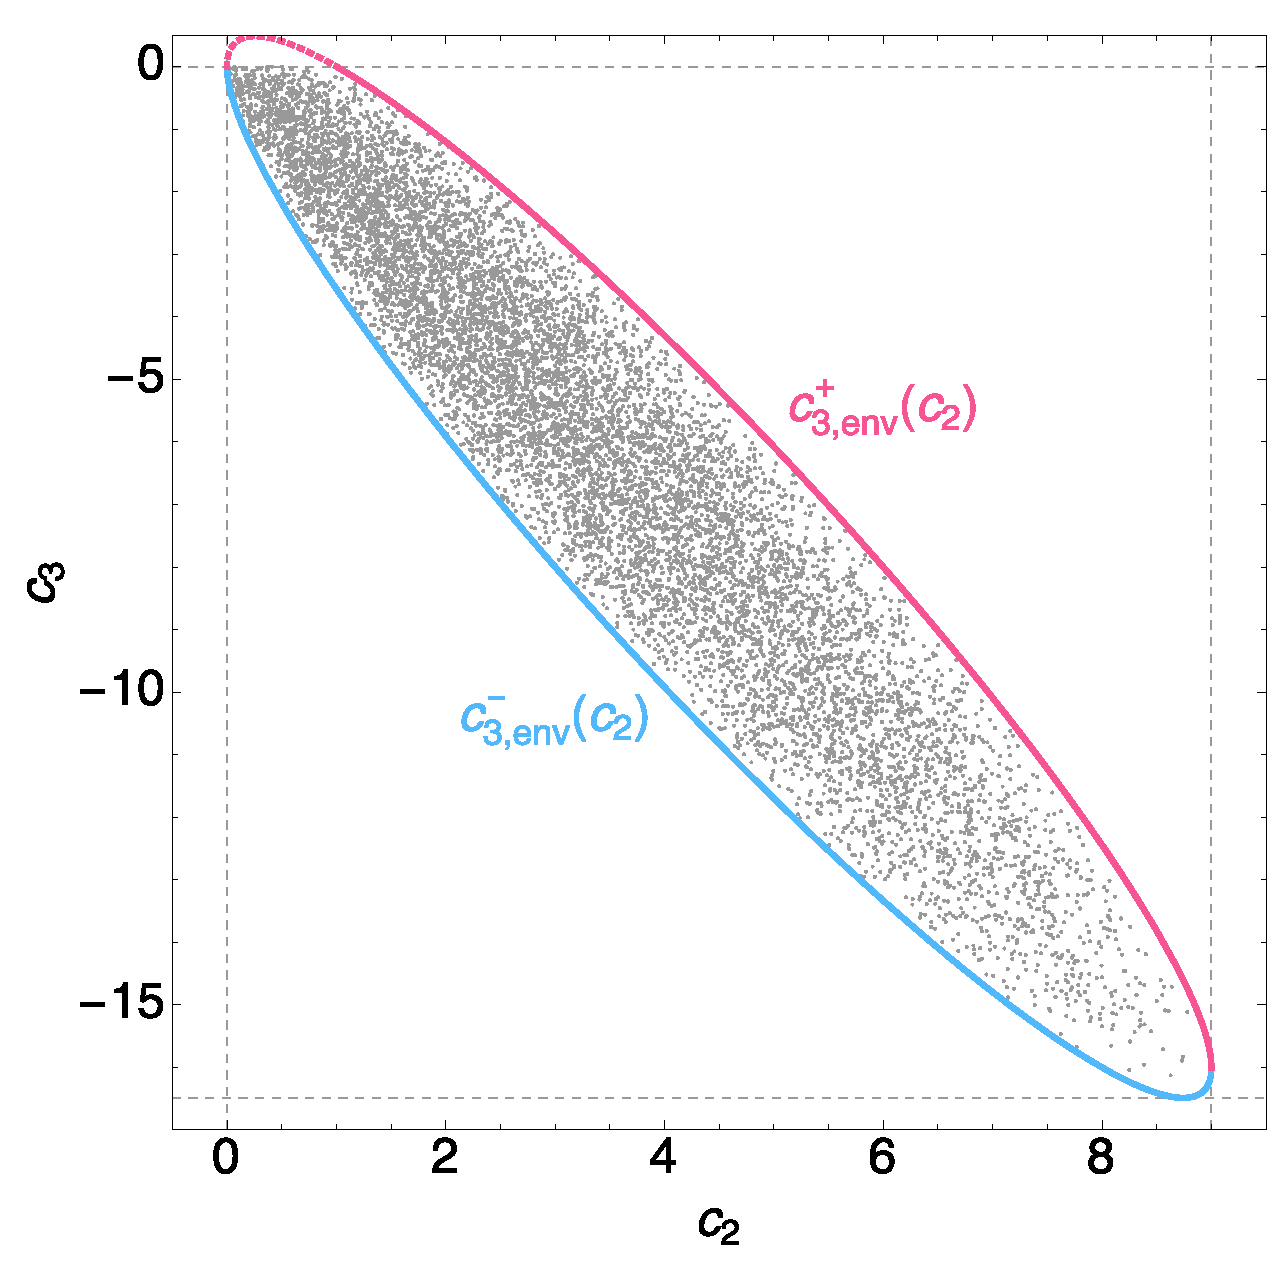
\includegraphics[width=\columnwidth]{c3c2surface.eps}
\caption{
Loci of points satisfying criteria A-G, plotted in the $c_3$-$c_2$ plane.
The pink/blue lines are given by $c_{3,\mathrm{env}}^{\pm}$.
}
\label{fig:c3c2surface}
\end{figure}

Inspection of Fig.~\ref{fig:c3c2surface} reveals that the loci of points are
nearly perfectly enveloped by the functions $c_3=(4/9) (-4c_2 \pm \sqrt{2 c_2} 
\sqrt{9-c_2})$, with the exception of a small region prohibited by criterion E
($c_3<0$). The envelope function may be derived starting from criteria A and G,
as follows:

\begin{align}
c_4 &< 1 - c_3 - c_2,\,\,\mathbf{[A]}\nonumber\\
c_4 &> \frac{9 c_3^2}{32 c_2},\,\,\mathbf{[G]}\nonumber\\
\implies \frac{9 c_3^2}{32 c_2} &< 1 - c_3 - c_2.
\end{align}

which may be re-arranged to

\begin{align}
9 &\Big( c_3 - \frac{4}{9} \big(-4c_2 - \sqrt{2 c_2} \sqrt{9-c_2}\big) \Big) \nonumber\\
\times &\Big( c_3 - \frac{4}{9} \big(-4c_2 + \sqrt{2 c_2} \sqrt{9-c_2}\big) \Big) < 0
\end{align}

For the above to hold, then $c_3$ must be larger than one of the radicals but
always less than the other, giving two possible sets of envelope functions.
We define the first one as:

\begin{align}
c_3 > c_{3,\mathrm{env}}^{-}(c_2) = \frac{4}{9} (-4c_2 - \sqrt{2 c_2} \sqrt{9-c_2}), \\
c_3 < c_{3,\mathrm{env}}^{+}(c_2) = \frac{4}{9} (-4c_2 + \sqrt{2 c_2} \sqrt{9-c_2}).
\end{align}

In Fig.~\ref{fig:c3c2surface}, the pink line depicts 
$c_{3,\mathrm{env}}^{+}(c_2)$, whilst the blue line depicts 
$c_{3,\mathrm{env}}^{-}(c_2)$. This demonstrates that indeed our first guess for
the form of the solution is correct. In principal though, we note that an 
alternative solution is $c_{3,\mathrm{env}}^{+}(c_2)<c_3<
c_{3,\mathrm{env}}^{-}(c_2)$.

From Fig.~\ref{fig:c3c2surface}, one can see that there is a minimum allowed
$c_3$ value and a maximum $c_2$. The maximum $c_2$ coincides where the two
envelope functions meet, meaning that $\sqrt{2 c_2} \sqrt{9-c_2}=0$, giving
$c_2=9$. The minimum $c_3$ value can be found by minimizing the lower envelope,
which occurs at $c_2=(3/2)(3+2\sqrt{2})$, corresponding to the minimum value of
$c_3=-8-6\sqrt{2}$, or $-16.4853...$. This therefore provides two of the missing
three LDC bounds we seek.

\subsection{$c_4$-$c_2$ plane}
\label{sub:c4c2plane}

We may repeat this exercise in the $c_4$-$c_2$ plane, and the resulting loci
are shown in Fig.~\ref{fig:c4c2surface}. As before, two lines appear to 
nearly perfectly envelope the loci of points, which can be derived starting from
criteria A and G:

%%% c4-c2 surface
\begin{figure}
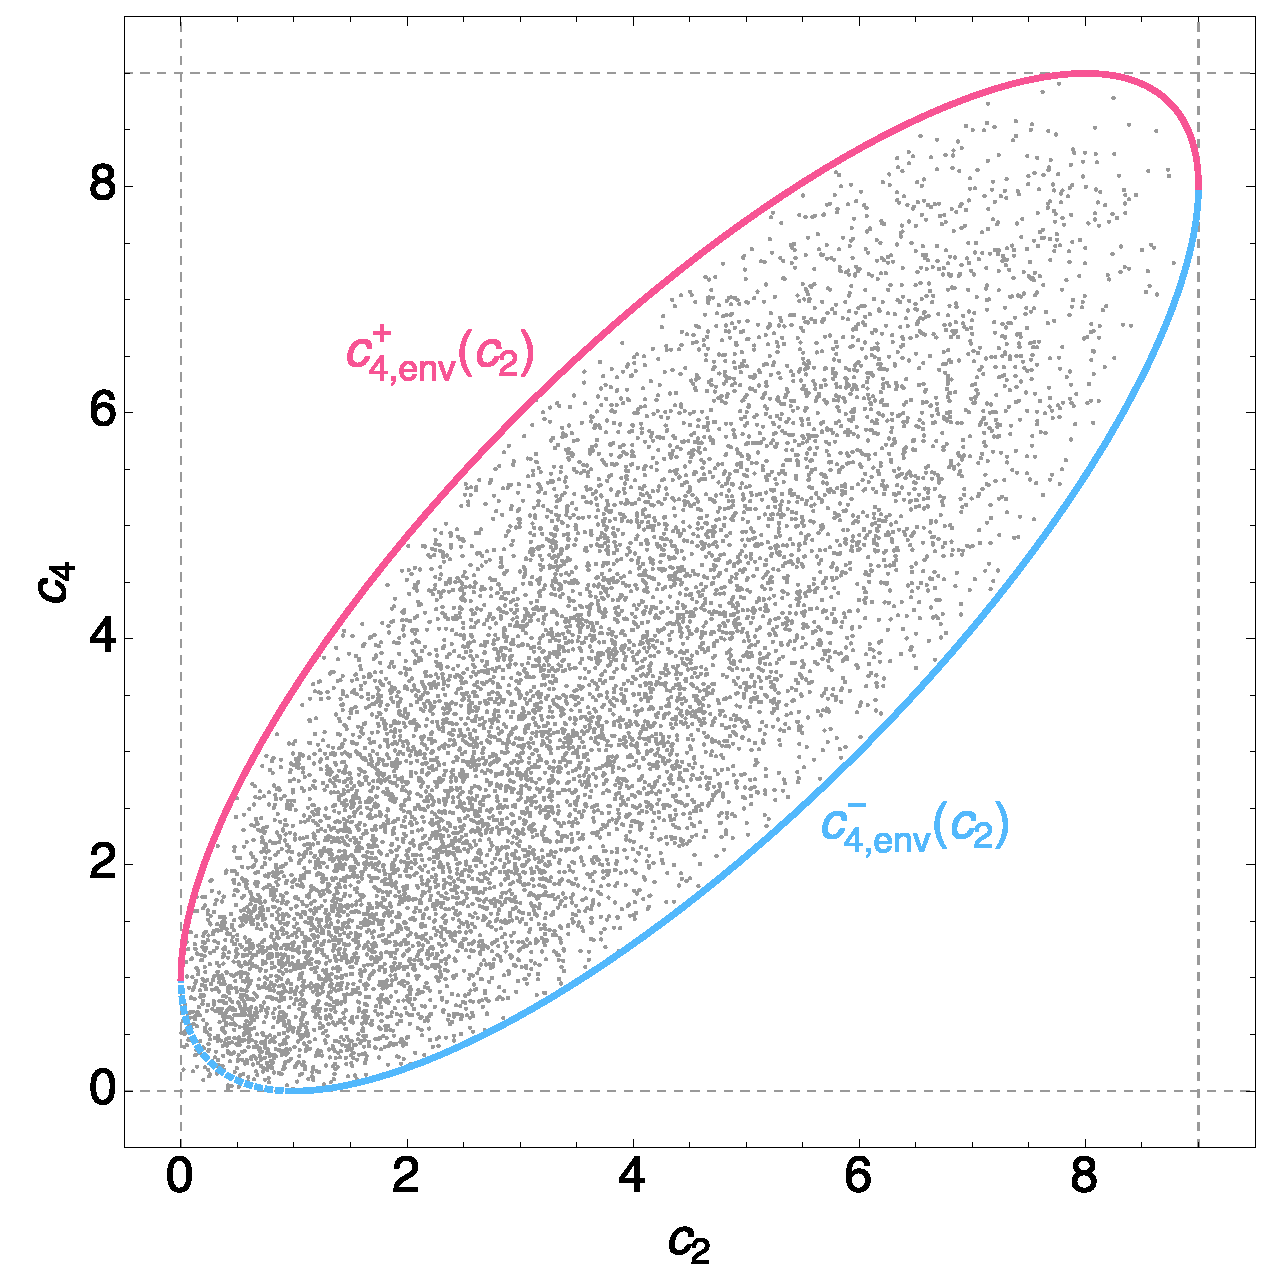
\includegraphics[width=\columnwidth]{c4c2surface.eps}
\caption{
Loci of points satisfying criteria A-G, plotted in the $c_4$-$c_2$ plane.
The pink/blue lines are given by $c_{4,\mathrm{env}}^{\pm}(c_2)$.
}
\label{fig:c4c2surface}
\end{figure}

\begin{align}
c_3^2 &> (c_2 + c_4 - 1)^2,\,\,\mathbf{[A]}\nonumber\\
c_3^2 &< \frac{32 c_4 c_2}{9},\,\,\mathbf{[G]}\nonumber\\
\implies (c_2 + c_4 - 1)^2 &< \frac{32 c_4 c_2}{9},
\end{align}

where the last line may now be re-expressed as

\begin{align}
&\Big( c_4 - \frac{1}{9} \big( 9 + 7c_2 - 4\sqrt{2 c_2} \sqrt{9-c_2} \big) \Big) \nonumber\\
\times &\Big( c_4 - \frac{1}{9} \big( 9 + 7c_2 + 4\sqrt{2 c_2} \sqrt{9-c_2} \big) \Big) < 0
\end{align}

The above requires that $c_4$ is greater than one of the radicals but always 
less than the other. Therefore, we have two valid envelope functions and we 
define the first one as:

\begin{align}
c_4 > c_{4,\mathrm{env}}^{-}(c_2) = \frac{1}{9} \big( 9 + 7c_2 - 4\sqrt{2 c_2} \sqrt{9-c_2} \big), \\
c_4 < c_{4,\mathrm{env}}^{+}(c_2) = \frac{1}{9} \big( 9 + 7c_2 + 4\sqrt{2 c_2} \sqrt{9-c_2} \big),
\end{align}

These two functions envelope the loci of points simulated earlier. This is 
apparent from Fig.~\ref{fig:c4c2surface}, where the pink line denotes 
$c_{4,\mathrm{env}}^{+}(c_2)$ and the blue line $c_{4,\mathrm{env}}^{-}(c_2)$. 
We plot the $c_{4,\mathrm{env}}^{-}(c_2)$ function from the upper-right 
intersection down to hitting the $c_4$ boundary condition of criterion F. 
Extending the line further back, shown as a dotted line, does not provide a 
physical bound on the points, although we note that only a very small fraction 
of points are excluded by doing so. In any case, the objective here is merely to
determine the upper limit on $c_4$.

We may use the $c_{4,\mathrm{env}}^{+}(c_2)$ function to find the maximum 
bound on $c_4$. Maximizing the $c_{4,\mathrm{env}}^{+}(c_2)$ function 
by differentiation, we find the curve is maximized at $c_2=8$, corresponding to
$c_4 = 9$. This provides the last limit needed to define the cuboid containing 
all loci as tightly as possibly:

\begin{align}
0 < c_2 < 9,\nonumber\\
-8-6\sqrt{2} < c_3 < 0,\nonumber\\
0 < c_4 < 9.
\end{align}

\subsection{$c_4$-$c_3$ plane}
\label{sub:c4c3plane}

Although we have now derived all of the LDC bounds, for the sake of 
completeness we here consider envelope functions bounding the $c_4$-$c_2$ plane, 
as shown in Fig.~\ref{fig:c4c3surface}.

%%% c4-c3 surface
\begin{figure}
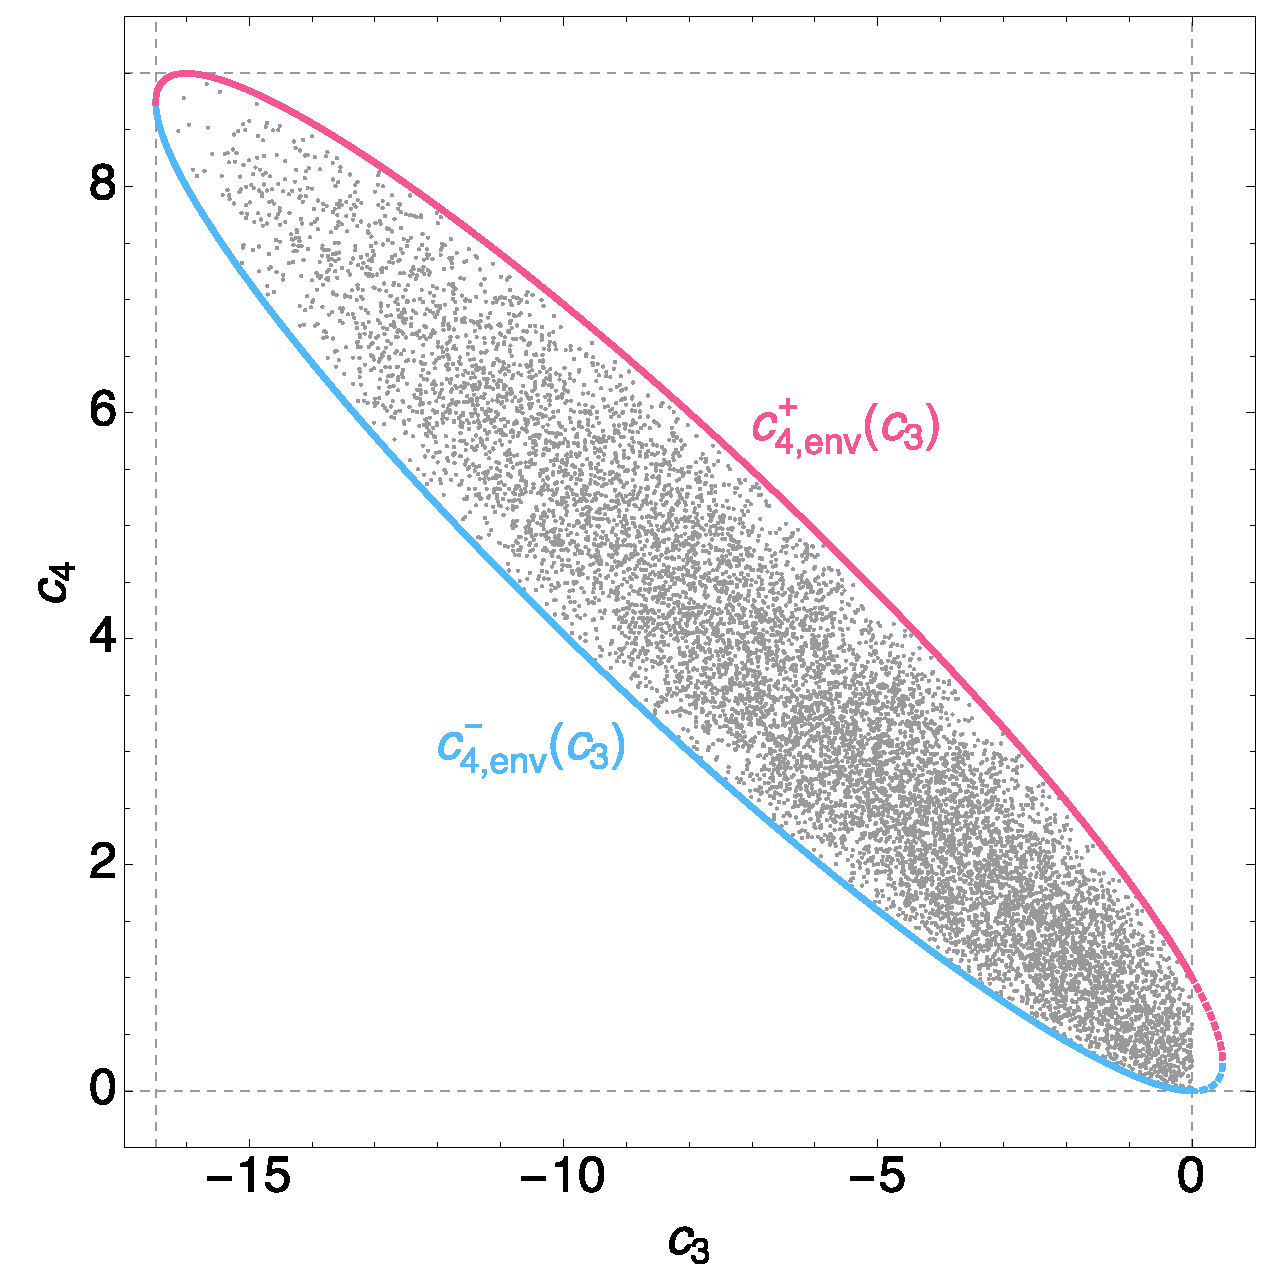
\includegraphics[width=\columnwidth]{c4c3surface.eps}
\caption{
Loci of points satisfying criteria A-G, plotted in the $c_4$-$c_3$ plane.
The pink/blue lines are given by $c_{4,\mathrm{env}}^{\pm}(c_3)$.
}
\label{fig:c4c3surface}
\end{figure}

The pink and blue lines shown in Fig.~\ref{fig:c4c3surface} nearly perfectly
envelope the loci of allowed points, with the exception of criterion 
E ($c_3<0$) truncating a small fraction of points. As before, these functions
may be derived from the following:

\begin{align}
c_2 &< 1 - c_3 - c_4,\,\,\mathbf{[A]}\nonumber\\
c_2 &> \frac{9 c_3^2}{32 c_4},\,\,\mathbf{[G]}\nonumber\\
\implies \frac{9 c_3^2}{32 c_4} &< 1 - c_3 - c_4,
\end{align}

which may be re-expressed as

\begin{align}
32 &\Big( c_4 - \frac{1}{8}\big( 4 - 4c_3 - \sqrt{2}\sqrt{8-16c_3-c_3^2} \big) \Big) \nonumber\\
\times&\Big( c_4 - \frac{1}{8}\big( 4 - 4c_3 + \sqrt{2}\sqrt{8-16c_3-c_3^2} \big) \Big) < 0.
\end{align}

Following the lines of argument used before, this provides the envelope 
functions:

\begin{align}
c_4 > c_{4,\mathrm{env}}^{-}(c_3) = \frac{1}{8}\big( 4 - 4c_3 - \sqrt{2}\sqrt{8-16c_3-c_3^2} \big), \\
c_4 < c_{4,\mathrm{env}}^{+}(c_3) = \frac{1}{8}\big( 4 - 4c_3 + \sqrt{2}\sqrt{8-16c_3-c_3^2} \big).
\end{align}

We note that the two functions meet when $\sqrt{8-16c_3-c_3^2}=0$, occurring
at $c_3 = -8 + 6 \sqrt{2} = 0.4853...$. However, criterion G truncates these
functions, albeit only a small fraction of the envelope.
